% =====================================================================
\chapter{Eredmények: a generátormodellek}
\label{ch:modellek}
% =====================================================================

Ez a fejezet a generátormodelleket veti össze: hogyan teljesít a három helyi modell azonos dokumentumokon,
mennyire közelíti meg egy helyi modell a nagy szervermodellt, miért bukott el a magyarra továbbtanított
PULI-LlumiX, és mekkora memóriát igényelnek a modellek. A modelleket kizárólag azonos dokumentumhalmazon
hasonlítjuk össze, és mindenhol megnevezzük, melyiken.

% =====================================================================
\section{A három helyi modell azonos dokumentumokon}
\label{sec:modellek-kozos}
% =====================================================================

\begin{sloppypar}
Két ilyen halmaz van:
\begin{enumerate}[label=(\alph*),leftmargin=*,itemsep=1pt,topsep=2pt]
\item Az előzetes vizsgálat hat dokumentumán (\code{en-economics-short-01},
\code{en-humanities-medium-02}, \code{en-law-long-03}, \code{hu-coffee}, \code{hu-gametheory},
\code{hu-immune}) a Qwen2.5-7B és a szervermodell futott; mivel ezek a fő vizsgálatban is szerepelnek, a
PULI-LlumiX és a Gemma eredménye ezekre leszűkítve is számolható (\ref{tab:modellek-kozos}.~táblázat).
\item A fő vizsgálat 30 dokumentumán a PULI-LlumiX és a Gemma futott.
\end{enumerate}
\end{sloppypar}

\begin{table}[htbp]
\centering
\caption{A generátormodellek minőségi indexe ($Q$) a hat közös dokumentumon.}
\label{tab:modellek-kozos}
\small
\setlength{\tabcolsep}{4.5pt}
\begin{tabular}{@{}lcccccl@{}}
\toprule
 & \multicolumn{3}{c}{Helyi generátormodellek ($Q$)} & \multicolumn{2}{c}{Wilcoxon-$p$} & \\
\cmidrule(lr){2-4}\cmidrule(lr){5-6}
Konfiguráció & \makecell{Qwen2.5\\7B} & \makecell{PULI-\\LlumiX 8B} & \makecell{Gemma 3\\12B} & \makecell{Qwen--\\PULI} & \makecell{Qwen--\\Gemma} & \makecell[l]{Szerver\\($Q$, konfig.)} \\
\midrule
\multicolumn{7}{@{}l}{\emph{Alapvonalak}} \\
\arm{B-doc-L} & 0,83 & 0,49 & \cellcolor[HTML]{E6F4EA}\textbf{0,97} & 0,031 & 0,031 & 0,95 (\arm{B-doc-S}) \\
\arm{E0}      & 0,64 & 0,32 & \cellcolor[HTML]{E6F4EA}\textbf{0,71} & 0,031 & 0,094 & 0,94$^a$ (\arm{E4}) \\
\midrule
\multicolumn{7}{@{}l}{\emph{A módszer lépései}} \\
\arm{E1}      & 0,88 & 0,59 & \cellcolor[HTML]{E6F4EA}\textbf{0,95} & 0,031 & 0,22  & -- \\
\arm{E2}      & \cellcolor[HTML]{E6F4EA}\textbf{0,96} & \cellcolor[HTML]{E6F4EA}\textbf{0,72} & \cellcolor[HTML]{E6F4EA}\textbf{0,97} & 0,063 & 0,66  & 1,00$^a$ (\arm{E4b}) \\
\arm{E3}      & 0,88 & 0,44 & \cellcolor[HTML]{E6F4EA}\textbf{0,97} & 0,031 & 0,22  & -- \\
\midrule
\multicolumn{7}{@{}l}{\emph{Kiegészítő ablációk}} \\
\arm{E2f}     & 0,90 & 0,69 & \cellcolor[HTML]{E6F4EA}\textbf{0,98} & 0,031 & 0,094 & -- \\
\arm{E2h}     & 0,92 & 0,63 & \cellcolor[HTML]{E6F4EA}\textbf{0,96} & 0,063 & 0,094 & -- \\
\arm{E2x}     & 0,89 & 0,71 & \cellcolor[HTML]{E6F4EA}\textbf{0,96} & --    & --    & -- \\
\midrule
\multicolumn{7}{@{}l}{\emph{Darabolási változatok}} \\
\arm{E5a}     & 0,87 & 0,36 & \cellcolor[HTML]{E6F4EA}\textbf{0,97} & 0,031 & 0,031 & -- \\
\arm{E5b}     & 0,70 & 0,23 & \cellcolor[HTML]{E6F4EA}\textbf{0,76} & 0,031 & 0,31  & -- \\
\arm{E5c}     & 0,86 & 0,29 & \cellcolor[HTML]{E6F4EA}\textbf{0,97} & 0,031 & 0,69  & -- \\
\bottomrule
\end{tabular}

\smallskip
\parbox{\textwidth}{\footnotesize\textbf{Jelmagyarázat:} A hat közös dokumentum az előzetes vizsgálat dokumentumhalmaza (a PULI-LlumiX 8B és a Gemma 3 12B értéke a fő vizsgálat futásaiból, erre a hat dokumentumra leszűkítve). \emph{Wilcoxon-$p$:} páros Wilcoxon-próba a hat dokumentumon, korrigálatlan, leíró jellegű (hat dokumentumon a legkisebb elérhető érték $0{,}031$). \emph{Szerver:} a szervermodell ugyanazzal a konfigurációval (\arm{B-doc-S}, \arm{E4}, \arm{E4b}). $^a$Csak a három közös angol dokumentumon. Kiemelés (\colorbox[HTML]{E6F4EA}{\textbf{félkövér}}): soronként a legjobb helyi modell (mindenütt a Gemma 3 12B), illetve oszloponként az adott helyi modell saját csúcsértéke.}
\end{table}

A három helyi modell erősorrendje minden vizsgált dokumentumhalmazon következetes:
\begin{itemize}[leftmargin=*,itemsep=2pt,topsep=2pt]
\item \emph{A hat közös dokumentumon (3 magyar, 3 angol):} a sorrend minden konfigurációban Gemma $>$ Qwen $>$ PULI. A Qwen a PULI-nál nyolc konfigurációban mind a hat dokumentumon jobb ($p=0{,}031$), az \arm{E2}-ben és az \arm{E2h}-ban pedig $p=0{,}063$ mellett. A Gemma minőségi indexe mindenütt magasabb a Qwenénél, de mind a hat dokumentumon egyöntetű előnyt csak a teljes dokumentumos promptnál ($0{,}83$ vs.\ $0{,}97$, a legnagyobb különbség) és az \arm{E5a}-nál mutat ($p=0{,}031$); a különbség az \arm{E2}-nél a legkisebb ($0{,}96$ vs.\ $0{,}97$, $p=0{,}66$).
\item \emph{A három saját magyar szövegen:} a magyarra továbbtanított PULI a magyar szövegeken is a leggyengébb maradt (\arm{E2}: Qwen $0{,}96$, PULI $0{,}74$, Gemma $0{,}97$; \arm{E0}: Qwen $0{,}88$, PULI $0{,}39$, Gemma $0{,}99$).
\item \emph{A fő vizsgálat 30 dokumentumán:} a Gemma mind a tíz összevetett konfigurációban szignifikánsan felülmúlja a PULI-t (páros Wilcoxon-próba, korrigálatlanul $p\le5{,}3\cdot10^{-6}$; értékek: \ref{tab:fo}.~táblázat). A különbség az \arm{E2}-nél a legkisebb ($0{,}67$ vs.\ $0{,}95$), az \arm{E5c}-nél pedig a legnagyobb ($0{,}25$ vs.\ $0{,}97$): a tervezett folyamat csökkenti a modellek közötti távolságot, de nem tünteti el.
\end{itemize}

% =====================================================================
\section{A szervermodell és a helyi modellek}
\label{sec:modellek-szerver}
% =====================================================================

A szervermodell (az egyetemi GenAI-szerver nagy Qwen-modellje) csak az előzetes vizsgálatban futott; a helyi Qwen2.5-7B-vel való összevetését \az{\ref{tab:szerver-helyi}}.~táblázat foglalja össze. Hat, illetve három dokumentumon ezek leíró jellegű eredmények (\ref{sec:statisztika}.~szakasz); a megosztott szerveren mért futási időket a helyiekkel nem vetjük össze (a szerver saját \arm{E4b}/\arm{E4} időszorzója kb.\ $9\times$).

\begin{table}[htbp]
\centering
\caption{A helyi Qwen2.5-7B és a szervermodell összevetése az előzetes vizsgálatban.}
\label{tab:szerver-helyi}
\small
\setlength{\tabcolsep}{2pt}
\begin{tabular}{@{}llcccccc@{}}
\toprule
Folyamat & Modell (konfig.) & $Q$ (6 dok.) & \makecell{$Q$ (3 angol\\dok.)} & \makecell{Elsőre\\átment} & \makecell{„Felhasz-\\nálnám”} & \makecell{Bloom-\\egyezés} & \makecell{Lefedett-\\ség} \\
\midrule
\multirow{2}{*}{Teljes dok.}
  & Qwen2.5-7B (\arm{B-doc-L}) & 0,83 (0,76--0,90) & -- & -- & 68\,\% & -- & 45\,\% \\
  & Szerver (\arm{B-doc-S})    & 0,95 (0,87--0,99) & -- & -- & --     & -- & --     \\
\midrule
\multirow{2}{*}{Naiv RAG}
  & Qwen2.5-7B (\arm{E0})      & 0,64 (0,46--0,81) & 0,40 & -- & 34\,\% & -- & 25\,\% \\
  & Szerver (\arm{E4})         & 0,91 (0,80--0,98)$^a$ & 0,94 & -- & -- & -- & 9\,\%  \\
\midrule
\multirow{2}{*}{\makecell[l]{Tervezett +\\ellenőrzött}}
  & Qwen2.5-7B (\arm{E2})      & \cellcolor[HTML]{E6F4EA}\textbf{0,96} (0,93--0,98) & \cellcolor[HTML]{E6F4EA}\textbf{0,95} & 23\,\% & 80\,\% & 35\,\% & 44\,\% \\
  & Szerver (\arm{E4b})        & \cellcolor[HTML]{E6F4EA}\textbf{0,99} (0,97--1,00)$^a$ & \cellcolor[HTML]{E6F4EA}\textbf{1,00} & 83\,\% & 98\,\% & 62\,\% & 28\,\% \\
\bottomrule
\end{tabular}

\smallskip
\parbox{\textwidth}{\footnotesize\textbf{Jelmagyarázat:} $Q$ (6 dok.): minőségi index a hat dokumentumon (zárójelben a helyi modellnél a 95\,\%-os konfidenciaintervallum, a szervermodellnél a dokumentumonkénti terjedelem). $^a$A szervermodell \arm{E4} és \arm{E4b} konfigurációja a saját hat angol dokumentumán futott; a helyi modellel való közvetlen összevetés a három közös angol dokumentumon lehetséges.}
\end{table}

Az összevetésből három fő tanulság adódik:
\begin{itemize}[leftmargin=*,itemsep=2pt,topsep=2pt]
\item \emph{A helyi modell a módszerrel eléri a szerveres alapvonalakat:} a helyi Qwen2.5-7B a tervezett és ellenőrzött folyamattal (\arm{E2}, $Q=0{,}96$) a hat közös dokumentumon eléri a szervermodell teljes dokumentumos promptját (\arm{B-doc-S}, $0{,}95$), a három közös angol dokumentumon pedig a szervermodell naiv RAG-ját ($0{,}95$ vs.\ $0{,}94$). Ugyanezzel a módszerrel azonban a szervermodell is tovább javul (\arm{E4b}: $0{,}99$, a három közös angol dokumentumon $1{,}00$), így a „helyi modell eléri a szervermodellt” állítás kizárólag a szerveres alapvonalakra igaz.
\item \emph{A tervezett folyamatban a szervermodell a részmutatókon is fölényben van:} az \arm{E4b}-ben a kérdéshelyek 83\,\%-a elsőre átment az ellenőrzésen (Qwen \arm{E2}: 23\,\%), a bíró „felhasználnám” aránya 98\,\% (Qwen: 80\,\%), a tervezett és megvalósult Bloom-szint pedig az esetek 62\,\%-ában egyezett (Qwen: 35\,\%).
\item \emph{A naiv RAG hibáit a nagy szervermodell sem kerüli el:} az \arm{E4} konfigurációban a kérdéspárok 49\,\%-a közel azonos volt, a dokumentum-lefedettség mindössze 9\,\%-ot ért el (\arm{E4b}: 28\,\%), és a modell tartalmilag üres kérdéseket is írt („Hány szóból áll a »Link to Learning« cím?”), amelyeket a bíró 5/5-re pontozott -- ugyanaz a rövid szerkezeti darab vitte félre, mint a helyi naiv RAG-ot (\ref{sec:fo-robusztus}.~szakasz).
\end{itemize}

% =====================================================================
\section{Miért bukik el a PULI-LlumiX?}
\label{sec:fo-puli}
% =====================================================================

A magyarra továbbtanított modelltől azt vártuk, hogy a magyar dokumentumokon jobb lesz a többnyelvű
modelleknél; ehelyett a magyar szövegeken is a leggyengébb lett, és ennek oka az \emph{utasításkövetés}. A
modellkártya szerint a PULI-LlumiX-Llama-3.1 a Llama 3.1 8B \emph{Instruct} modell magyar szövegeken folytatott
további előtanítása, utólagos utasítás-hangolás nélkül (a kártya „base” modellnek nevezi)~\cite{pulillumix}; a
vizsgálatban egy harmadik féltől származó, GGUF-kvantált változat futott
({\small\nolinkurl{hf.co/mradermacher/PULI-LlumiX-Llama-3.1-GGUF:Q4_K_M}}).

Egyetlen hívásban a PULI a kért tíz kérdés helyett átlagosan 1,8-at (\arm{E0}), illetve 5,6-ot (\arm{B-doc-L})
adott vissza; az egyhívásos konfigurációk vizsgáinak 94--99\,\%-a formailag hibás volt, a darabolási változatok
vizsgáinak 14--29\,\%-ában a válasz nem is volt értelmezhető JSON. A tervezett folyamat ezt részben megkerüli,
mert hívásonként egy kérdést kér, de ott is konfigurációnként 128--620 modellválasz volt értelmezhetetlen (a
Gemmánál és a Qwennél egy sem). Az ellenőrzés nélküli \arm{E1} kérdéseinek 34\,\%-a szivárogtatja a kulcsot,
45\,\%-ának törzse nem kérdés, a kérdéspárok 62\,\%-a közel azonos, a törzsek átlagosan 252 karakteresek (a Gemma
\arm{E1}-ében 122): a modell jellemzően a forrás egy mondatát másolja be kérdésként és kulcsként is
(\ref{sec:szivargas}.~szakasz). A \emph{Nürnbergi per} című cikk esetén például a generált „kérdés” egy kijelentő forrásmondat
volt, a négy válasz közül kettő ugyanezt a mondatot ismételte, a bíró helyességi pontszáma pedig 1/5 lett. Az ellenőrző lánc a szivárgást
(34\,\%$\to$12\,\%) és a nem kérdő törzseket (45\,\%$\to$22\,\%) mérsékli, de a megvalósult Bloom-szint
gyakorlatilag mindig az emlékezés marad, és a teljes módszerrel is 18 dokumentumon $0{,}70$ alatt marad a
minőségi index (a leggyengébben $0{,}38$). Az \arm{E1} futása instabil is volt: 103 modellhívás időtúllépéssel
vagy hibával zárult, a medián vizsgaidő 96 perc lett (a Gemmánál 2,9 perc).

Fontos hangsúlyozni, hogy ez a megállapítás kizárólag a vizsgált modellváltozatra vonatkozik: a kudarcot nem
maga a magyar nyelvű továbbtanítás okozta, hanem az, hogy a további előtanítást nem követte újabb
utasításhangolás, így a modell nem tartotta be a strukturált kimeneti formátumot. Feltevésként a GGUF-fájlba ágyazott csevegési sablon (chat-sablon) is szerepet
játszhatott; ezt nem vizsgáltuk, és a kvantálás hatását sem tudjuk elkülöníteni.

% =====================================================================
\section{Memóriaigény és futási idő}
\label{sec:fo-eroforras}
% =====================================================================

\Az{\ref{tab:eroforras}}.~táblázat a modellek mért memóriaigényét, \az{\ref{fig:minoseg-ido}}.~ábra a minőséget
a futási idő függvényében mutatja.

\begin{table}[htbp]
\centering
\caption{A helyi generátormodellek memóriaigénye és relatív futási ideje.}
\label{tab:eroforras}
\small
\begin{tabular}{@{}lcccc@{}}
\toprule
Modell & Modell (GiB) & Teljes dok.\ (GiB) & Kártya & \arm{E2}/\arm{E0} \\
\midrule
Qwen2.5-7B (Q4\_K\_M)     & 4,8 & 5,2 & 8\,GB-os           & 10,9$\times$ \\
PULI-LlumiX 8B (Q4\_K\_M) & 5,5 & 6,5 & 8\,GB-os$^\ast$    & 52,3$\times$ \\
Gemma 3 12B (Q4\_K\_M)    & 7,8 & 7,8 & 12\,GB-os          & 8,5$\times$ \\
\bottomrule
\end{tabular}

\smallskip
\parbox{\textwidth}{\footnotesize\textbf{Jelmagyarázat:} \emph{Modell (GiB):} az Ollama által jelentett, mért foglalás 8\,192 tokenes kontextusnál (a \ref{tab:budget}.~táblázat becslésével összevetendő). \emph{Teljes dok.\ (GiB):} ugyanez a 16\,384 tokenes \arm{B-doc-L} konfigurációnál. \emph{Kártya:} a szükséges fogyasztói GPU az asztali környezet 1,6--1,9\,GiB-os foglalása mellett (a pilot mérése). \emph{\arm{E2}/\arm{E0}:} a medián vizsgaidő modellen belüli szorzója ugyanazon a kártyán (\ref{tab:koltseg}.~táblázat). $^\ast$A 16\,384 tokenes teljes dokumentumos konfigurációhoz a 8\,GB-os kártya várhatóan nem elég (lásd a szöveget).}
\end{table}

\paragraph{Memória.} A Qwen2.5-7B és a PULI-LlumiX 8B 8\,192 tokenes kontextussal egy 8\,GB-os fogyasztói
kártyán is elfér (a pilot RTX 3070 Ti-ján a Qwennel a legrosszabb esetben is kb.\ 380\,MiB tartalék maradt); a
Gemma 3 12B foglalása az asztali környezettel együtt kb.\ 9,4--9,7\,GiB, vagyis 12\,GB-os kártyát igényel. A
16\,384 tokenes konfigurációnál a Qwen foglalása 464\,MiB-tal nőtt, nagyságrendben egyezően a \eqref{eq:vram}
becslés 448\,MiB-os KV-többletével; a PULI-é 1\,024\,MiB-tal, így az asztali környezettel együtt meghaladná egy
8\,GB-os kártya kapacitását (fogyasztói kártyán ezt nem mértük). A Gemma foglalása gyakorlatilag nem nőtt
(16\,MiB), feltehetően a csúszóablakos helyi figyelemrétegek miatt~\cite{gemma3}; ezt nem vizsgáltuk.

\paragraph{Futási idő.} A szorzókat egy vizsgálaton belül értelmezzük (\ref{sec:fo-koltseg}.~szakasz). A PULI
$52{,}3\times$-os szorzója félrevezetően nagy, mert az \arm{E0}-ja alig ír kérdést; a fő vizsgálaton belül,
azonos dokumentumokon és kártyán a PULI \arm{E0}-ja a Gemmáénak kb.\ 0,4-szerese, az \arm{E2}-je viszont kb.\
2,4-szerese, mert szinte minden kérdéshelyet újra kell próbálnia (2,0 kísérlet a Gemma 1,3-ával szemben,
\ref{tab:ellenorzo}.~táblázat), és sok válasza értelmezhetetlen. A Qwen idejét a fő vizsgálat modelljeiével nem
vetjük össze, mert más vizsgálatban, más dokumentumokon mértük. A mérések alapján két GPU-szint különíthető el:
8\,GB-on a 7--8B modellek (a vizsgált feladatra ezek közül a Qwen2.5-7B alkalmas), 12\,GB-on a Gemma 3 12B, amely
minden konfigurációban a legjobb helyi eredményt adta.

\begin{figure}[htbp]
\centering
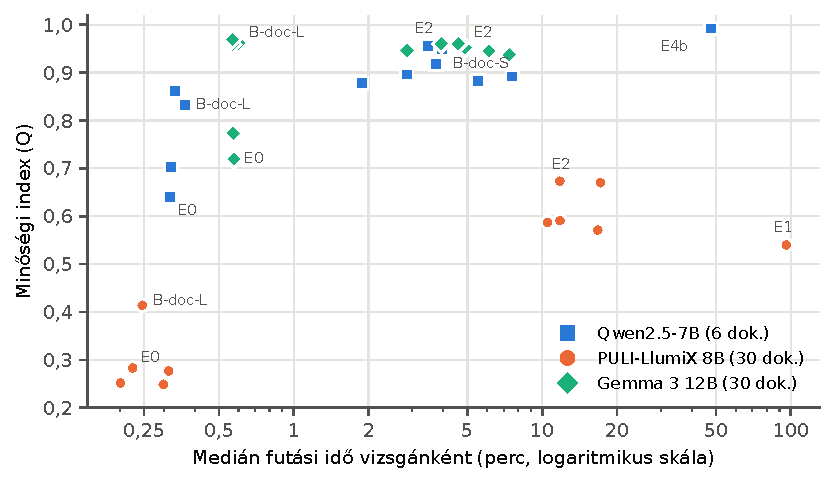
\includegraphics[width=0.85\textwidth]{figures/f4_minoseg_ido}
\caption[Minőség és futási idő.]{Minőség és futási idő. Az egyhívásos konfigurációk gyorsak, de minőségük a
modelltől és a darabolástól függően erősen ingadozik; a tervezett konfigurációk lassabbak, de minden modellnél a
legjobbak között vannak. A Qwen2.5-7B az előzetes vizsgálat hat dokumentumán, a másik két helyi modell a fő
vizsgálat 30 dokumentumán, a szervermodell (\arm{B-doc-S}, \arm{E4b}) pedig megosztott szerveren futott, ezért az
abszolút időtengely modellen belül értelmezendő (a relatív időszorzókat \az{\ref{tab:koltseg}}.~táblázat adja).}
\label{fig:minoseg-ido}
\end{figure}

% =====================================================================
\section{Modellválasztási tanulság}
\label{sec:modellek-tanulsag}
% =====================================================================

A vizsgált feladatban az utasításkövetés fontosabb volt a nyelvi specializációnál: a többnyelvű Qwen2.5-7B a hat
közös dokumentumon, a magyar szövegeken is, minden konfigurációban jobb volt a magyarra továbbtanított
PULI-LlumiX 8B-nél. Minél erősebb a modell, annál kisebb a módszer haszna a minőségben: ugyanezen a hat
dokumentumon az \arm{E2}--\arm{E0} különbség a PULI-nál $0{,}41$, a Qwennél $0{,}32$, a Gemmánál $0{,}26$, az
\arm{E2}--\arm{B-doc-L} különbség $0{,}23$, $0{,}12$, illetve nulla; az erős modellnél a módszer értéke ezért
elsősorban az ellenőrizhetőség, a gyenge modellnél maga a használható vizsga. Mivel ezt a modellkártya nem mutatja
meg, a modellt a célfeladaton mérve kell kiválasztani.
